\section{System Design and Responsibilities}

The Moving Object Pipeline System has two main responsibilities: the
generation and maintenance of the Moving Object database, and the
prediction of known object locations which are sent to the Association
Pipeline to prevent unneccessary alerts.  The MOPS has been broken
into two components, colloquially known as ``DayMOPS'' and ``NightMOPS.''
 

\begin{figure}[!ht]
\centering
  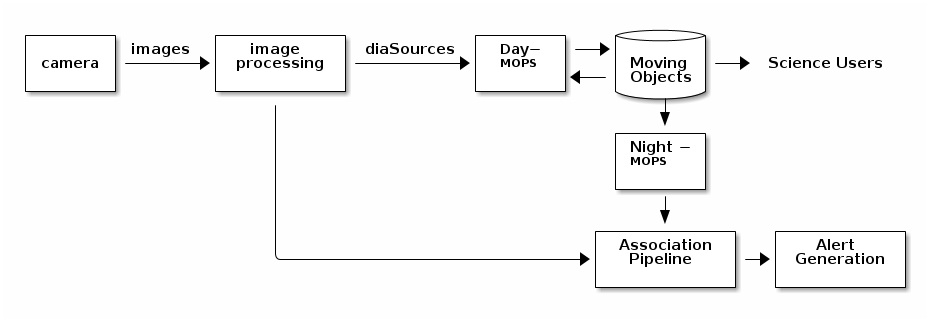
\includegraphics[width=13cm]{illustrations/mopsWithinLsst.png}
\caption{ Data flow from the camera through DayMOPS to the Science
  Users and Alert Generation.  DayMOPS will build and maintain the
  Moving Objects table, NightMOPS will use the Moving Objects table to
  communicate with the Assocation Pipeline.  }
\label{mopsWithinLsst}
\end{figure}


``DayMOPS,'' so called because it processes data acquired from the
previous night in a large batch operation, is responsible for
discovering new Moving Objects in newly-acquired data, searching old
data for detections of new objects, and updating the Moving Objects
table to reflect newly-acquired data. It is also responsible for
periodically cleaning and refining the contents of the Moving Objects
table.  ``NightMOPS'' is responsible for projecting the locations of known
Moving Objects in upcoming images as they are announced during
night-time operations.  

The relationship between DayMOPS, NightMOPS and the neighboring
components of the LSST Data Management system is illustrated in
figure \ref{mopsWithinLsst}.

\subsection{DayMOPS: Discovering and Managing Moving Objects}

% Illustration of DayMOPS

% sky-plane vs. orbit-space illustration

The DayMOPS is responsible for discovering moving objects in source
catalogs.  The task of discovering unknown asteroids has a very
lengthy history, involving human, electronic, and computerized actors.

From the beginning the primary detectable feature of an asteroid is
it's motion across the sky as time progresses -- which makes the
underlying orbital parameters of critical relevance to the continued
tracking of the object.  The first asteroid, Ceres, was visually
detected by Piazzi \citep{1802QB378} through its motions
against the background star as he attempted to verify the position of
a star in a published catalog.  Without knowing how orbits were
goverened, Piazzi's initial tracking effort involved constant repeated
night-to-night observations which he was only able to maintain for a
limited time due to his health and the motion of the asteroid into the
daytime sky.  It fell to Carl Friedrich Gauss to develop his method of
orbit determination before Ceres could be recovered again thus firmly
establishing the mathematics of orbits as a required prerequisite.

Optical observations had their limitations, however, and the archival
record created by the application of photography to observations was
of critical importance to scientific demands of repeatability.  The
first photographic discovery of an asteroid, (323) Brucia, was by Max
Wolf in 1891 \citep{1892AN} as he recognized the
non-sidereal rate trails on his photographs for the asteroids they
were.  Wolf became a prolific discoverer of asteroids (almost 250
total) through photography and as such developed the standard
detection technique used for the next century.

Photographic sensitivity is determined to a large part through
exposure time and asteroid motion to first order is a function of its
distance so two main types of photographic survey methodology were
used.  Surveys looking for closeby and fast near-Earth asteroids (like
those of \cite{1988NASTM4041...52S}) used non-sidereal trailed motions
and generally shorter exposure times.  A discovered trail of any
length in the and image developed in an observatory darkroom would
lead to additional exposures of the asteroid being quickly acquired
and the data required to secure the orbit.  The second technique,
useful for very slow moving asteroids that did not appear as a trailed
images was to take several exposures and then manually alternate
between them rapidly, thus depending on the well-developed human
motion sense to discover the moving asteroids.  Machines were built
for this purpose, such as the blink comparator.  Besides its use for
stellar proper motions, this technique's most well known success was
in the discovery of Pluto by Tombaugh \citep{1960S&T....19..264T}.
The blink comparator was useful for scientific studies of asteroids in
the main asteroid belt such as the seminal Palomar-Leiden survey
\citep{1970A&AS....2..339V}.  Keeping the exposure times short was
important to keep the asteroid images starlike so their isophotal
diameter could be used inaccurate brightness calibration.  This
allowed for the rapid discovery of asteroids for the time: 2400
discoveries in 11 nights of observation.

The advent of the CCD was applied to asteroids early, with the long
readout times (and consequential 50\% duty cycle) minimized through
the process of drift scannings.  Gehrels and the Spacewatch Project
\citep{1990ASPC....8...51G} pioneered the use of CCD's in the
detection of asteroids, making the first CCD detection of the
near-Earth asteroid 1989 UP and the first discovery as well (1990 SS).
Spacewatch went on to built an advanced real time asteroid motion
detection program, MODP \citep{1991AJ....101.1518R}.  Drift scanning
was made unnecessary by the advent of large format cameras used in a
step-and-stare mode such as that of the NEAT project
\citep{1999AJ....117.1616P}.  With the introduction of custom
frame-transfer CCD's and high-capacity computer processing, the LINEAR
project \citep{2000Icar..148...21S} and the Catalina Sky Survey
\citep{2007IAUS..236..323L} were able to progress handily towards the
Spaceguard goal.

As with photography, there are multiple techniques which can be
applied to CCD images to discover their asteroids.  Most asteroid
detection software uses a "moving target indicator" approach in that
CCD images are searched automatically for their objects who are then
compiled as a detection list.  By filtering out objects which did not
move and searching for asteroid-like motions in the unmatched lists,
motion candidates are created.  However, a more exotic approach called
Matched Filter Processing \citep{2005AJ....130.1951G} can be applied
that has several advantages.  Images are coadded rapidly along
hypothesized motion vectors.  If the flux of an object appears to grow
after coaddition, it becomes a candidate moving object with the motion
vector already determined.  This approach becomes computationally
expensive with a large number of possible motion vectors but has the
advantage of being able to detect fainter objects in the same set of
images compared to the moving target indicator approach.  It has been
used successfully in searches for distant objects such as those in the
Kuiper Belt \citep{BG, MB} and has been used to do NEA searches over
large portions of the sky where the asteroid is uncertain but has a
relatively small range of possible velocities
\citep{2005AJ....130.1951G}.

The advent of large-format all sky surveys have radically changed the
detection requirements both in terms of techniques for imagery and
software...  heheheh, all yours Jon.  I could only make mistakes in
this part of the discussion.


The design of the LSST DayMOPS is based on the PanSTARRS Moving Object
Pipeline System \citep{psMOPSDesign}.  The approach used here is to
first find sets of detections with sky-plane paths consistent with
asteroid behaviour; these sets of detections and their fitted paths
are called \textbf{tracks}.  A set of algorithms for the discovery of
sky-plane tracks in dense data are presented in
\citet{Kubica:2005:MTA:1081870.1081889}; these algorithms are the
basis of the linking methods for the current LSST DayMOPS.


%% TBD: it would be really nice to have some illustrations here
%% showing detections of an object, and possibly tracklets and tracks
%% as well

The tracking methods used are based on a tiered approach; first two or
more detections from a single night are linked into
\textbf{tracklets}, which represent a hypothetical object and a linear
approximation of its sky-plane motion.  These tracklets are later
joined into larger tracks. Because of the increasing complexity of
sky-plane motion over time, we are generally interested in tracks
which span no more than 15-30 days of observation time.

The PanSTARRS MOPS uses a fairly loose and generous approximation of
asteroid motion.  This allows for many mislinkages or \textbf{false
  tracks}, combining detections which are not attributable to the same
source, but virtually all objects for which a true (correctly-linked)
track could be generated will get some correct track.  With LSST's
expected density of detections, we found that this glut of false
tracks was generally too painful.  As a result, our methods diverge
from those of PanSTARRS as we introduce some more strict filters on
tracks, reducing the number of mislinkages at the expense of
potentially missing some true tracks.  The algorithms, their
implementations, the additional filters, and their behaviors are
presented thoroughly in Chapter \ref{linking}.

Once tracks are discovered, they are sent to the Orbit Determination
phase. The Orbit Determination phase takes these sets of sky-plane
detections and attempts to find a Keplerian orbit which could generate
the detections.  This orbit is further refined, and error bounds are
established, using differential correction.  Orbit Determination will
reject many tracks as false, but should successfully find precise
orbits for virtually all correctly linked tracks.  Several methods for
performing this task are known, and several have open-source implementations
available to LSST \citep{Milani04orbitdetermination},
\citep{Milani2006}, \citep{OpenOrb2009}, \citep{granvik_thesis}.  The
orbits discovered by Orbit Determination, and the detections present
in the track associated with each orbit, are used to generate new
Moving Objects.

\begin{figure}[h]
\begin{center}
  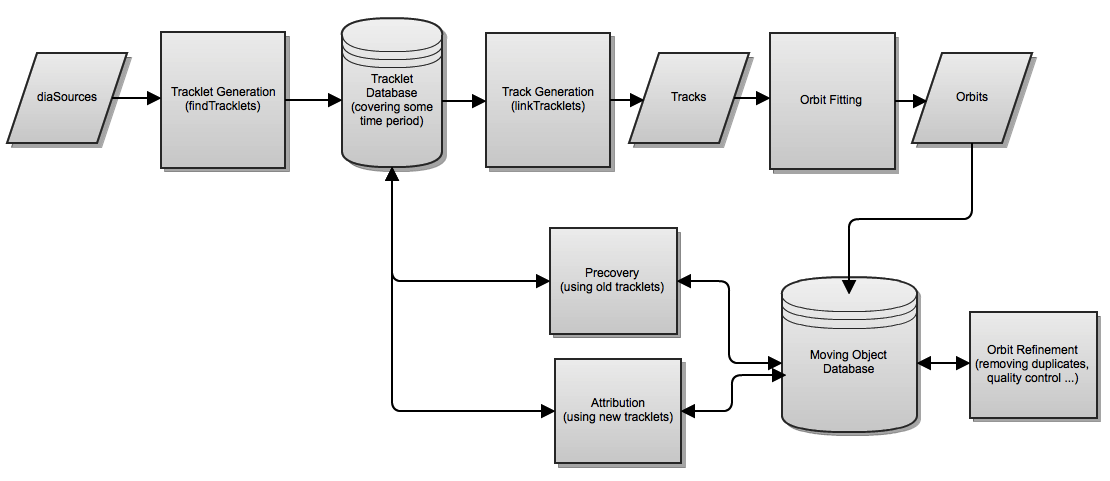
\includegraphics[width=11cm]{illustrations/mopsDiagram.png}
\end{center}
\caption{ Data flows into the DayMOPS pipeline and results in
  modifications of the Moving Objects table in a variety of ways,
  including attribution to known objects, a multi-stage pipeline for
  the discovery of new objects, and periodic refinements of the Moving
  Object table, such as possible merges of redundant objects or
  removal of false orbits. }
\label{mopsDiagram}
\end{figure}



The DayMOPS is expected to perform several additional tasks to manage
and improve the Moving Objects table over time.  Attribution is the
process of identifying known objects in incoming data and adding those
detections to the correct Moving Object, in a process called
Attribution. Similarly, Precovery is the recovery of known,
unattributed detections associated with a newly-discovered Moving
Object.  Another refinement is the merging of potentially redundant
Moving Objects.  The complete set of DayMOPS tasks and their data
flows are illustrated in figure \ref{mopsDiagram}.




